\documentclass[12pt,a4paper]{article}

%\usepackage{afterpage}
%$\usepackage{amsfonts}
\usepackage{amsmath}
%\usepackage{array}
\usepackage[backend=biber,style=apa,block=none]{biblatex}
\usepackage{booktabs}
\usepackage[skip=.5\baselineskip, font=footnotesize]{caption}
\usepackage{geometry}
\usepackage{graphicx}
\usepackage{parskip}
\usepackage{footnote}
%\usepackage{bigfoot}
\usepackage[hyperfootnotes=true]{hyperref}
%\usepackage{lmodern,textcomp}
%\usepackage{setspace}\onehalfspacing
%\usepackage{tabularx}
\usepackage[dvipsnames]{xcolor}
%\usepackage[symbol*]{footmisc}
\usepackage{eurosym}
\usepackage{makecell}
\usepackage{cleveref}

\graphicspath{{figures/}}
\addbibresource{references.bib}

\let\mkbibnamefamily\textsc

\geometry{top=2.25cm, bottom=2.5cm, left=3cm, right=2.5cm}
\hypersetup{colorlinks=true, linkcolor=blue, citecolor=blue, urlcolor=blue}
\captionsetup[figure]{labelfont=bf, singlelinecheck=off, justification=centering, labelsep=period}
\captionsetup[table]{labelfont=bf, singlelinecheck=off, justification=centering, labelsep=period}
\setlength{\skip\footins}{1cm}
\setlength{\footnotesep}{.5cm}

\begin{document}
\renewcommand{\thefootnote}{\fnsymbol{footnote}}
\begin{titlepage}
\newgeometry{top=3.5cm, bottom=2.5cm, left=3cm, right=2.5cm}
\begin{center}
    \LARGE
    \textbf{Twelve months after the Iberian exception:\\ A synthetic-controls estimation of its effects on inflation}
    \normalsize
    \vspace{1cm}
    \textbf{Miguel Haro Ruiz}\footnote{Corresponding author. E-mail address: m.haroruiz@gmail.com}\\
    \small
    Martin-Luther-Universität Halle-Wittenberg\\
    Große Steinstraße 73,\\
    06108 Halle (Saale),\\
    Germany\\
    \vspace{0.25cm}
    \normalsize
    \textbf{Christoph Schult}\\
    \small
    IWH – Halle Institute for Economic Research\\
    Kleine Märkerstraße 8,\\
    06108 Halle (Saale),\\
    Germany
    \vspace{0.25cm}
    \textbf{Christoph Wunder}\\
    \small
    Martin-Luther-Universität Halle-Wittenberg\\
    Große Steinstraße 73,\\
    06108 Halle (Saale),\\
    Germany\\
    \end{center}
    \vspace{0.75cm}
    \normalsize
    \textbf{Abstract}: This study employs synthetic control methods to estimate the effect of the Iberian exception mechanism on wholesale electricity prices and different aggregations of consumer inflation, for both Spain and Portugal. We find that the intervention achieved a 43\% reduction in the spot price of electricity in both Spain and Portugal between July 2022 and June 2023, with almost identical results. When considering the impact of the policy on inflation, the difference between the two countries is striking. On one hand, the effect on Spain's inflation is immediate and averages 3\% over the period under consideration. By contrast, the effect on Portugal’s price level kicks in with a six-month lag and amounts to a 1\% decline in overall CPI between January and June 2023. We argue that this divergence is explained by the different electricity retail contracts in each country. While the regulated tariff in Spain is directly indexed by wholesale prices, there is no direct link between wholesale and retail prices for Portugal in the short term.\par
    \textbf{Classification codes}: E31, L51, Q41, Q48
\end{titlepage}
\renewcommand{\thefootnote}{\arabic{footnote}}
\section{Introduction}\label{intro}
Among the array of policies implemented to counter the effects of the latest episode of energy-price inflation in Europe, the correction mechanism in the Iberian wholesale electricity market stands out as one of a kind.\footnote{\textbf{Abbreviations}: CP00: Overall CPI; CP00xNRG: Overall CPI excluding energy; DAA: Day-ahead auction; EC: European Commission; EU: European Union; IbEx: Iberian exception mechanism; MIBEL: Iberian Electricity Market; NRG: Energy CPI; SC: Synthetic controls.} By directly intervening in the day-ahead market, this policy earned the title of the Iberian exception mechanism (IbEx). The IbEx exploits the mechanics of the merit order auction, used to determine the day-ahead price of electricity. The policy imposes a cap on the price that gas generators can enter the auction with and outlines an adjustment mechanism to compensate for the losses that they incur when international gas prices are above the cap. As a result, gas generators are paid for their electricity at international gas prices, whereas other generators are paid for their electricity at a lower price than otherwise.\par 
This paper \textcolor{red}{contributes to a vast empirical literature analysing the interaction of energy markets on inflation and economic activity \parencite{clark2010time, baumeister2016forty, barsky2002oil, kilian2022impact}. In contrast to previous studies focusing on structural vector autoregressive models, we evaluate the effectiveness of the IbEx in reducing inflation by applying synthetic control (SC) methods.} By estimating reasonable counterfactual for Spain and Portugal, we find that the intervention reduced the day-ahead auction price of electricity by more than 40\% in both countries, with almost identical results. This had an immediate impact on Spain's overall inflation, which declined by 3\% over the first six months of the IbEx, an effect that can be traced back to a 20\% drop in energy-only inflation. In Portugal however, the effect of the IbEx took six months to spread onto consumers prices. In the six following months, overall inflation fell by 1\%, thanks to a 14\% reduction in the price of energy items. We argue that this divergence is explained by different contract types for electricity in the retail market in each country; While the regulated tariff in Spain is directly indexed by wholesale prices, there is no direct link between wholesale and retail prices in the short term for Portugal.\par 
\section{The Iberian Exception Mechanism}\label{ibex}
The Iberian Electricity Market (MIBEL) uses a market coupling algorithm to produce a single day-ahead price for Spain and Portugal. While the two countries share a wholesale market, their retail structures differ significantly. On one hand, Spanish consumers may choose to receive their electricity from retail providers or through the PVPC regulated tariff, which is directly indexed by MIBEL day-ahead prices and serves roughly 40\% of households and firms using up to 10kW of power \parencite{iea2021b}. By contrast, most Portuguese consumers source their electricity from private retailers and less than 5\% adhere to the regulated tariff, whose price is based on MIBEL prices from the previous year \parencite{iea2021a}.\par
The IbEx was approved by the governments of Spain and Portugal and entered into force on June 15, 2022. Under the intervention, regulators impose a limit, henceforth \textit{reference price}, on the price gas-fired electricity generators can enter the MIBEL day-ahead auction with. The \textit{reference price} was set at 40\euro/MWh during the first six months of the intervention and gradually increases in the months that follow. On days when international gas prices go above the \textit{reference price}, gas generators are entitled to adjustment payments. The adjustment cost results from comparing the \textit{reference price} to a daily gas \textit{market price} (\cite{boe2022}; \cite{diario2022}). The \textit{market price} is published daily before the day-ahead auction begins –such that market participants can submit their bids and offers with this knowledge– and is computed as a weighted average of gas contracts with maturity ranging between 1 and 3 days before the day under consideration \parencite{mibgas2022}. The adjustment cost is borne by market agents buying electricity indexed by the day-ahead auction price, and also financed through revenues from electricity exports to France.\par 

By introducing two prices –one for gas technologies and another one for the rest– the IbEx effectively decouples the price of electricity from international gas prices. While most countries across Europe have taken action to address the volatility in energy prices through direct transfers, energy taxes and VATs reductions as well as retail market regulations, the IbEx is the only measure that directly intervenes the spot price of electricity \parencite{sgaravatti2022}. The IbEx presents an ideal natural experiment to study its impact on inflation with causal implications. This is because, while MIBEL day-ahead market has been operating under special circumstances since June 15, all other European markets continue to follow the EU energy directives and guidelines in their integrity. However, the fact that only two units are treated under this intervention poses the fundamental challenge of finding an explicit counterfactual that can be used to estimate the effect of the policy.\par
\section{Methods}\label{methods}
The present study employs SC methods (\cite{abadie2003}; \cite{abadie2010}) to estimate the effect of the IbEx on a series of price outcome variables.\footnote{The estimation of SC units is done in R using the limSolve::lsei() function \parencite{soetaert2009}. Computation of p-values as well as of confidence intervals is done with the scinference package \parencite{wuthrich2021}.} The pool of control units includes 23 European countries,\footnote{All EU-27 countries plus Norway are considered, as they all operate under the EU Electricity Directives and the Guideline on Capacity Allocation and Congestion Management, as well as engage in market coupling through the Single Day-ahead Coupling mechanism. Cyprus and Malta are removed from the control pool because they do not operate a wholesale electricity market of their own. France is also removed, as we cannot rule out the possibility that the intervention affected its day-ahead electricity market \parencite{schlecht2022}.} and the treatment effect is estimated for each country separately i.e., Portugal is removed from the sample to estimate SC units for Spain, and vice versa. As outcome variables, we consider monthly average day-ahead prices (\cite{omie2022}; \cite{energycharts2022}) as well as three CPI aggregations at constant taxes; overall CPI (CP00), energy CPI (NRG), and Overall CPI excluding energy (CP00xNRG) \parencite{eurostat2023b}. This approach allows us to firstly, determine whether the IbEx had an effect on these inflation and secondly, to disaggregate the effect among energy and non-energy items.\par 
Following recommendations outlined by \textcite{ferman2020}, all our SC specifications include all pre-treatment outcome lags as predictors and the size of the pre-treatment period $T_0$ is large compared to that of the post-treatment period $T_1$. In particular, the results presented in the following section correspond to a specification where $T_0=108$ and $T_1=12$ months.\footnote{$T_0=89$ for day-ahead auction price due to lack of available data before 2015. Furthermore, Croatia, Hungary and Ireland are removed from the donor pool as their day-ahead price data is subject to inconsistencies.} To isolate the effect of the IbEx, only full-month intervention periods are considered, such that the post-intervention period goes from July 2022 to June 2023.\par
\section{Results}\label{results}
\begin{figure}[!h]
    \centering 
    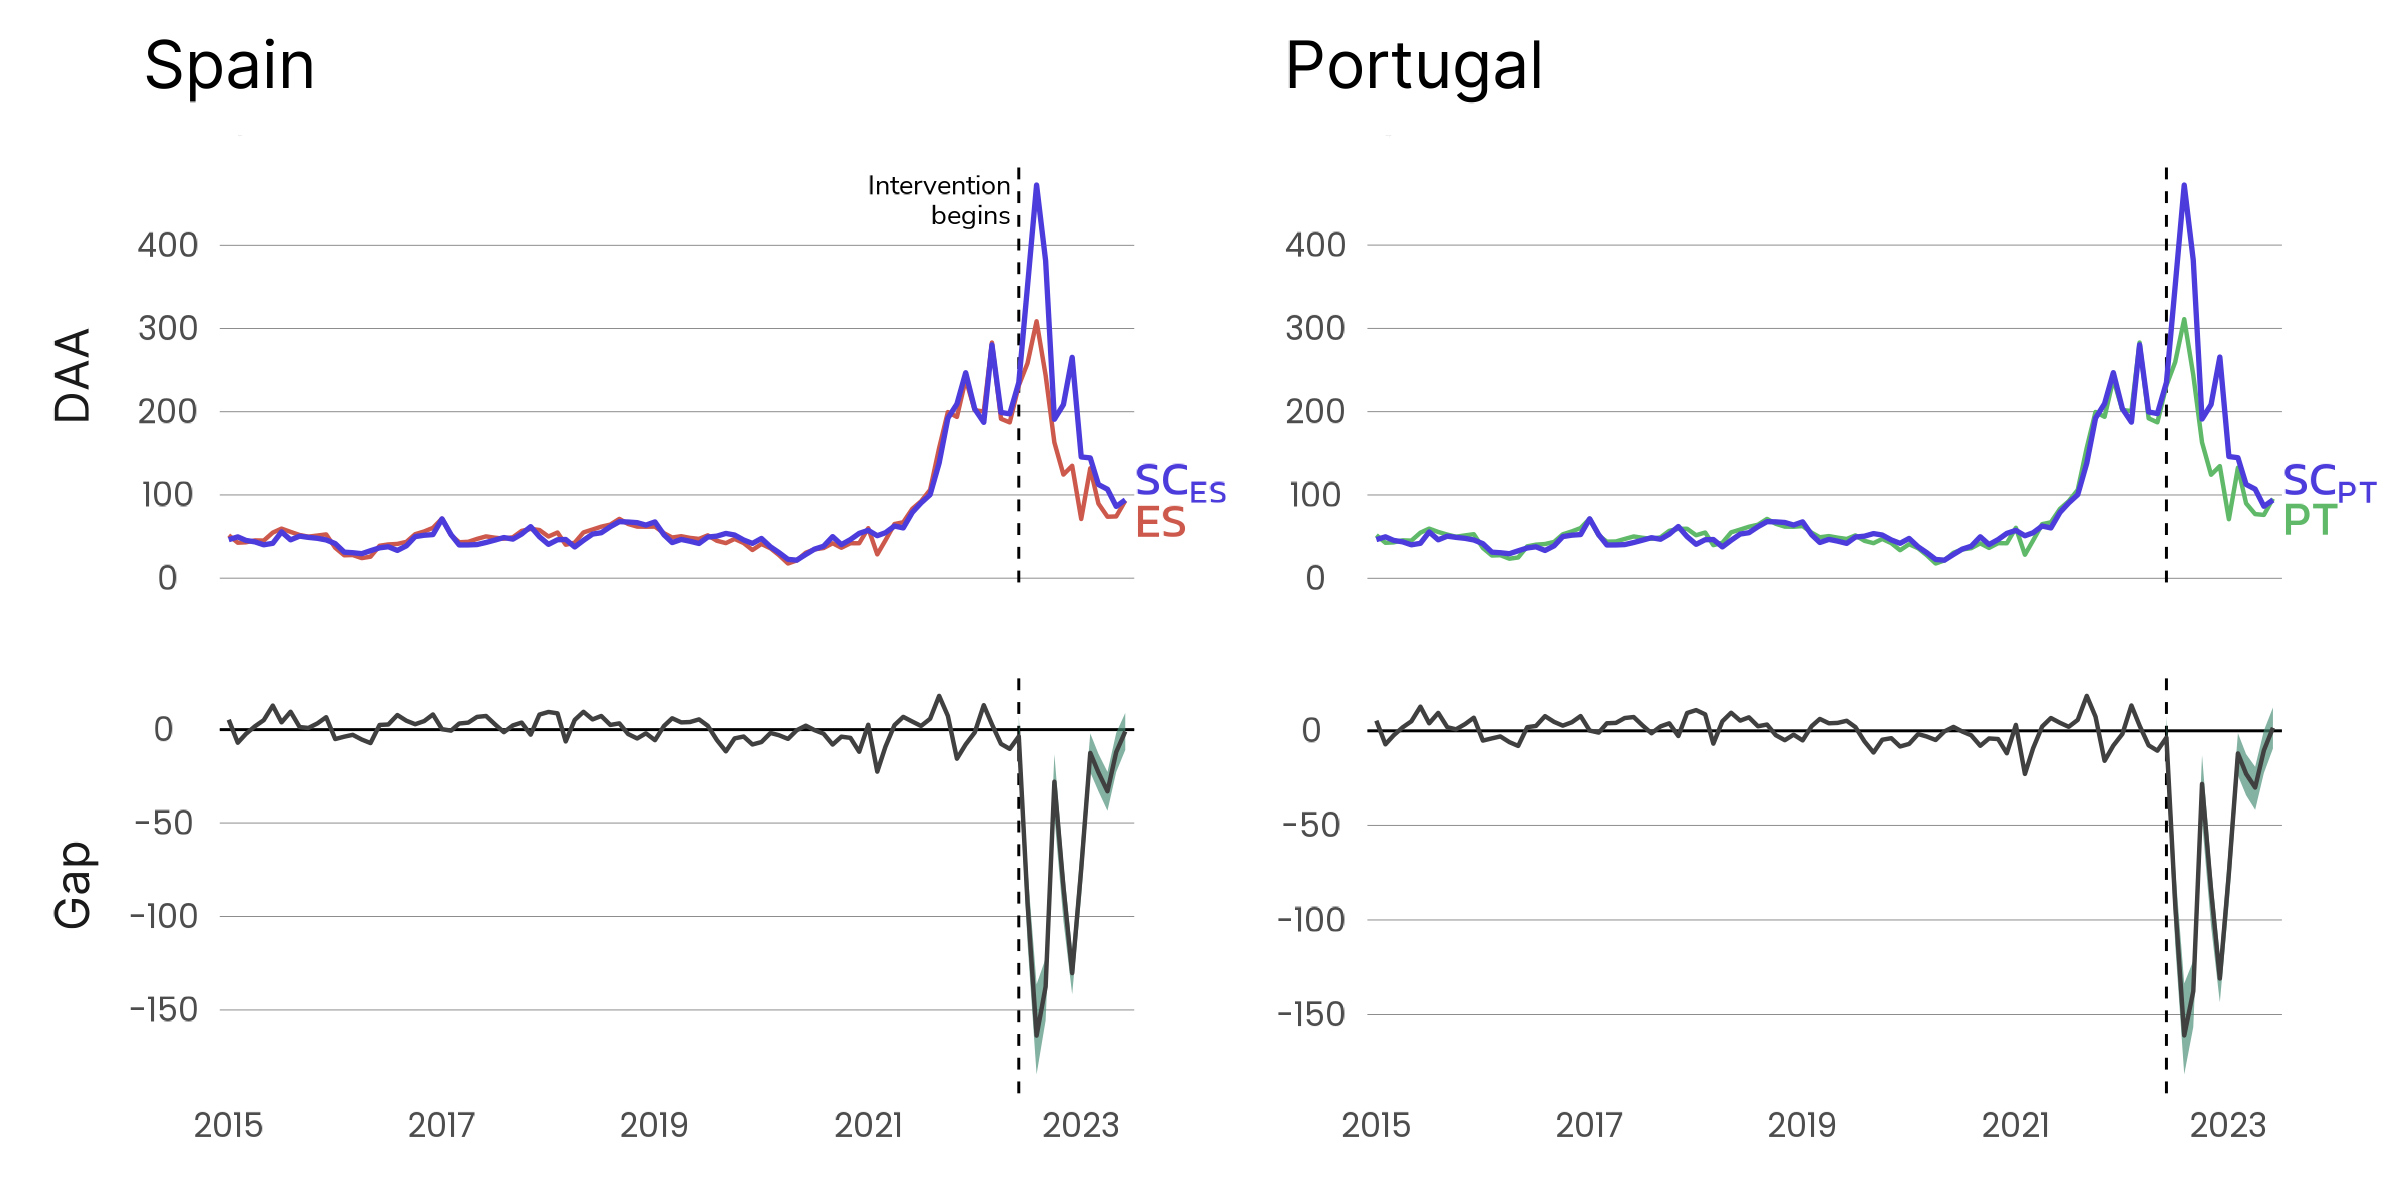
\includegraphics[width = .9\linewidth]{DAA_12.png}
    \caption{Observed and synthetic day-ahead price and difference between them with 90\% CI.}
    \label{fig:result_daa}
\end{figure}
Figure \ref{fig:result_daa} shows the effect of the IbEx on monthly day-ahead prices, resulting from the difference between the observed and synthetic trends for each country.\footnote{Refer to the \nameref{appendix} for the full results.} The estimated effect is almost identical in both countries, with an average decline in the price of 43\% between July 2022 and June 2023. Moving onto the impact on the energy CPI, figure \ref{fig:result_nrg} shows how the results vary significantly across the two treated countries. On one hand, the IbEx had an immediate and strong negative effect in Spain, particularly up to December 2022. Over its first twelve months, the intervention achieved a 19\% reduction in energy inflation . In the case of Portugal, the IbEx had virtually no effect on energy items up to December 2022. As soon as 2023 begins however, figure \ref{fig:result_nrg} shows a sharp decline of this indicators, which amounts to 14\% between January and December 2023.\par 
Overall, we have that IbEx had a stronger effect in Spain between July and December 2022 as overall inflation declined by 3\%. In Portugal the impact on overall CPI was only felt between January and December 2023, as indicated by a 1\% decline. The different results can be explained through differences in the retail market of electricity in each country. As described in section \ref{ibex}, the PVPC contract in Spain allows consumers to index their electricity bill by the spot price, creating a direct link between the day-ahead price and the energy CPI in the short term. By contrast, Portuguese retailers favor longer-term electricity contracts as price reference. As a result, it takes longer for retail prices to reflect consolidated changes in the wholesale market.\par
\begin{figure}[!h]
    \centering 
    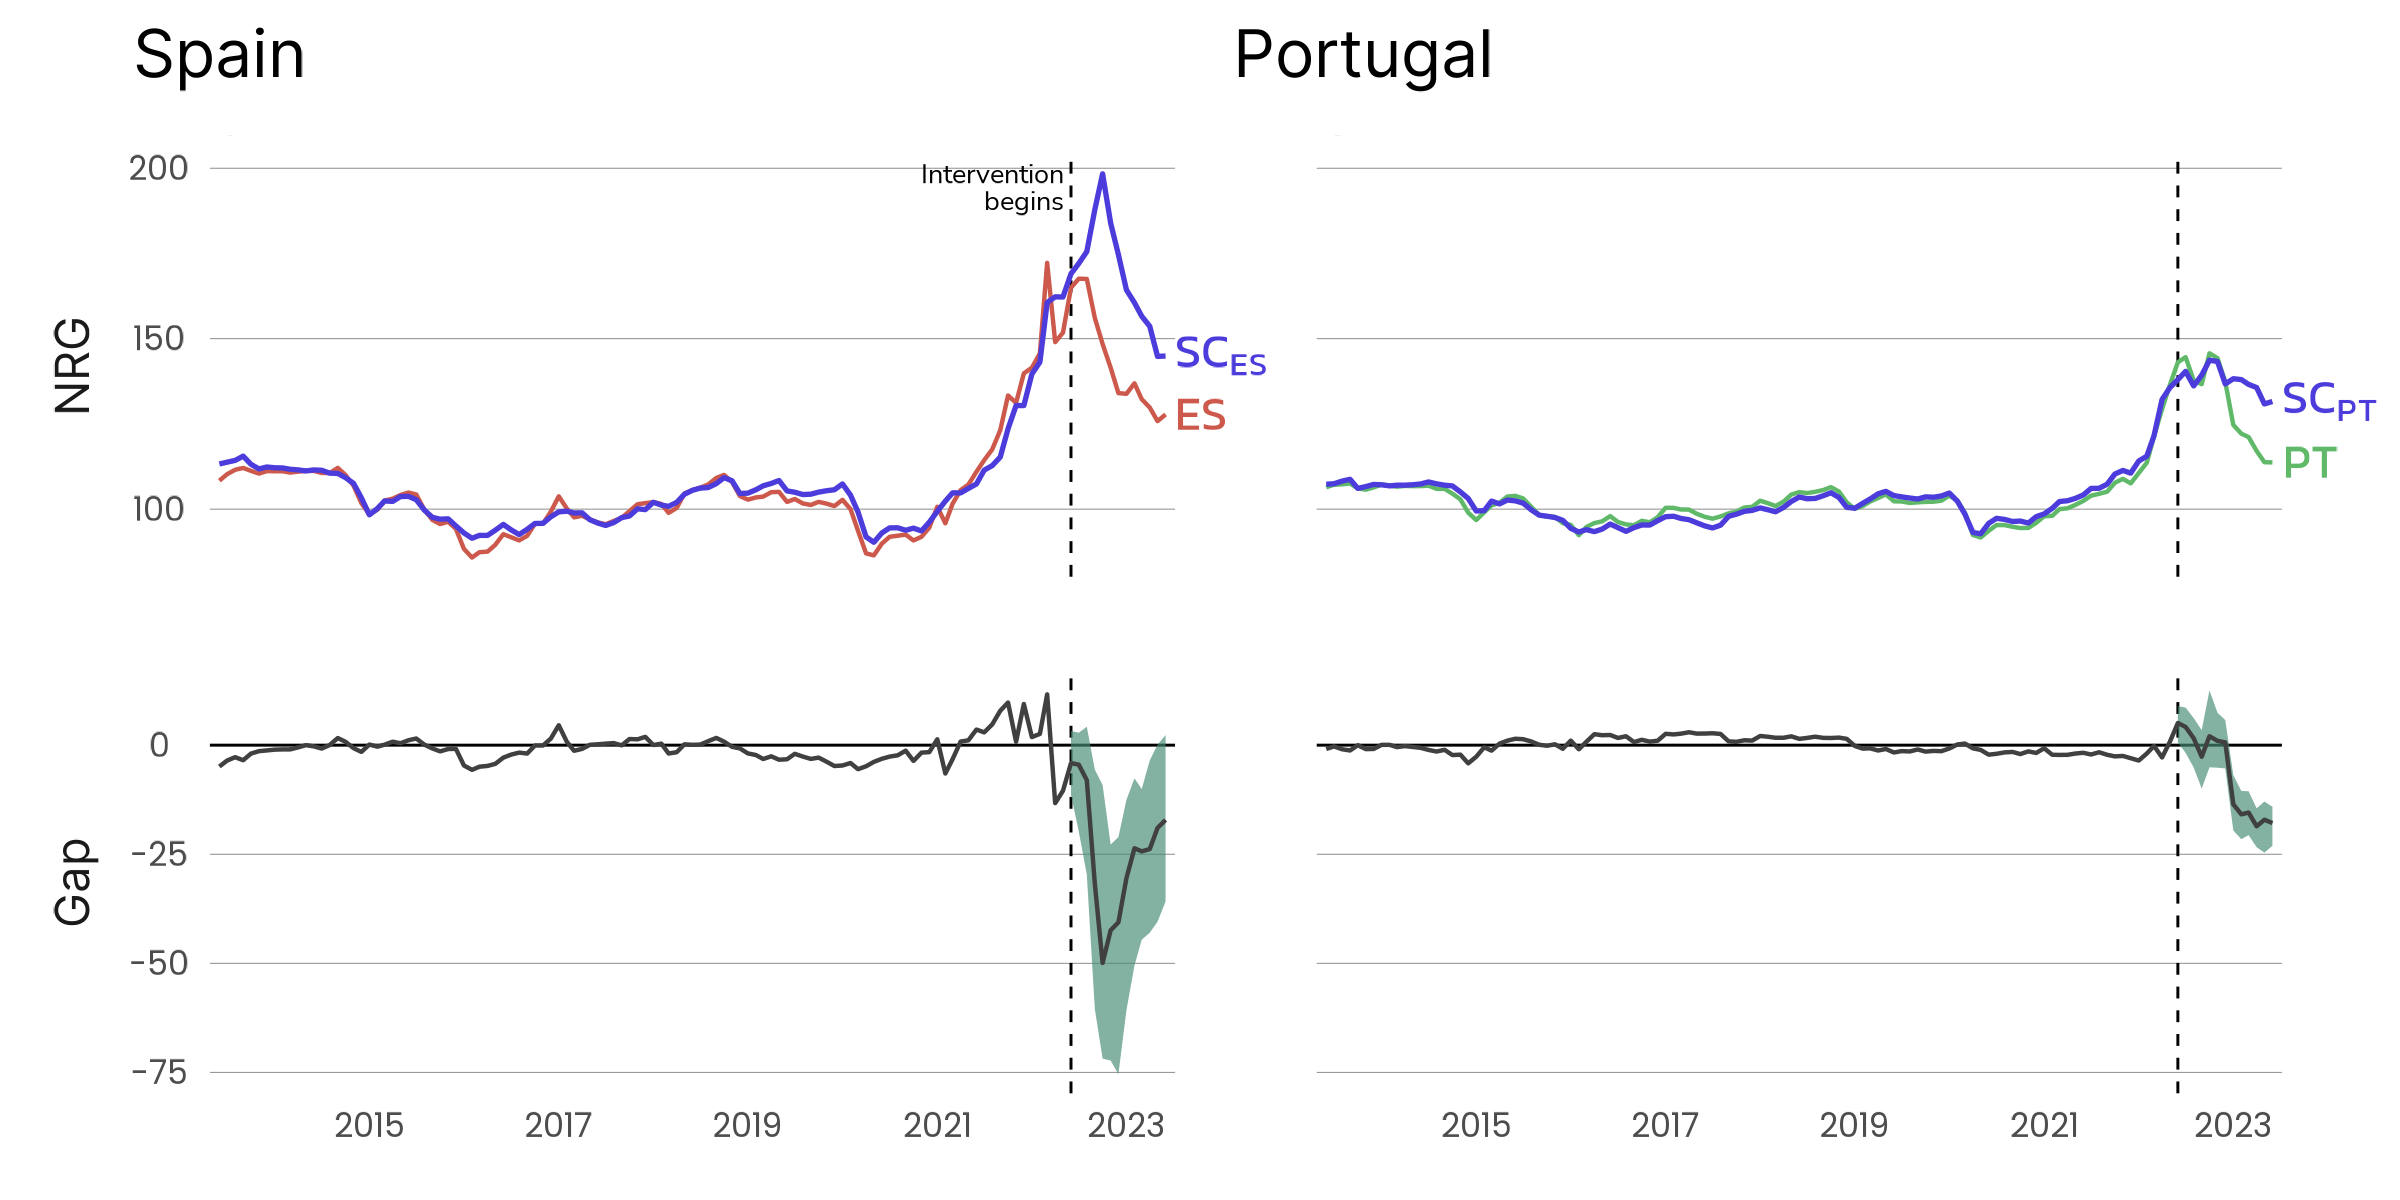
\includegraphics[width = .9\linewidth]{NRG_12_independent_y.png}
    \caption{Observed and synthetic energy inflation and difference between them with 90\% CI.}
    \label{fig:result_nrg}
\end{figure}
A relevant question that arises at this stage is how much of the reduction in the overall CPI is due to the direct impact of the IbEx on energy-only inflation, and how much can be explained by a reduction in the price of non-energy goods and services. Using the weights assigned to each CPI category \parencite{eurostat2023a}, we can disaggregate the effect on overall CPI among energy and non-energy items as follows:\par
\begin{align*}
\theta_{t}^{\mbox{\scriptsize{CP00}}}&=w_{t}^{\mbox{\scriptsize{NRG}}}\cdot\widehat{\theta}_{t}^{\mbox{\scriptsize{NRG}}}+w_{t}^{\mbox{\scriptsize{CP00xNRG}}}\cdot\widehat{\theta}_{t}^{\mbox{\scriptsize{CP00xNRG}}}\\
%&=0.117\cdot\widehat{\theta}_{t}^{\mbox{\scriptsize{NRG}}}+0.883\cdot\widehat{\theta}_{t}^{\mbox{\scriptsize{CP00xNRG}}}\\
&=\mbox{NRG}_{t}^{w}+\mbox{CP00xNRG}_{t}^{w}
\end{align*}
Where $w_{t}^{X}$ is the weight assigned to component $X$ of the CPI at time $t$, and $\widehat{\theta}_{t}^{X}$ is the effect of the IbEx on this component, estimated via SC. Figure \ref{fig:weighted_cp00_es} shows the decomposition of the effect on Spain’s overall CPI between energy and non-energy items.\footnote{The weights for Spain are .11748 (NRG) and .88252 (CP00xNRG) in 2022, and .90196 (NRG) and .09804 (CP00xNRG) in 2023} Between July and September 2022, the 9\% reduction in energy-only CPI caused by the IbEx fully explains the decline in overall inflation. In the nine months that follow, the reduction in the wholesale price of electricity spreads to non-energy items, whose CPI declines by 1.5\%. This decline is responsible for one-third of the reduction in overall CPI, whereas the remaining three-fourths correspond to a 22\% decline in the energy-only index.\par
\begin{figure}[!h]
    \centering 
    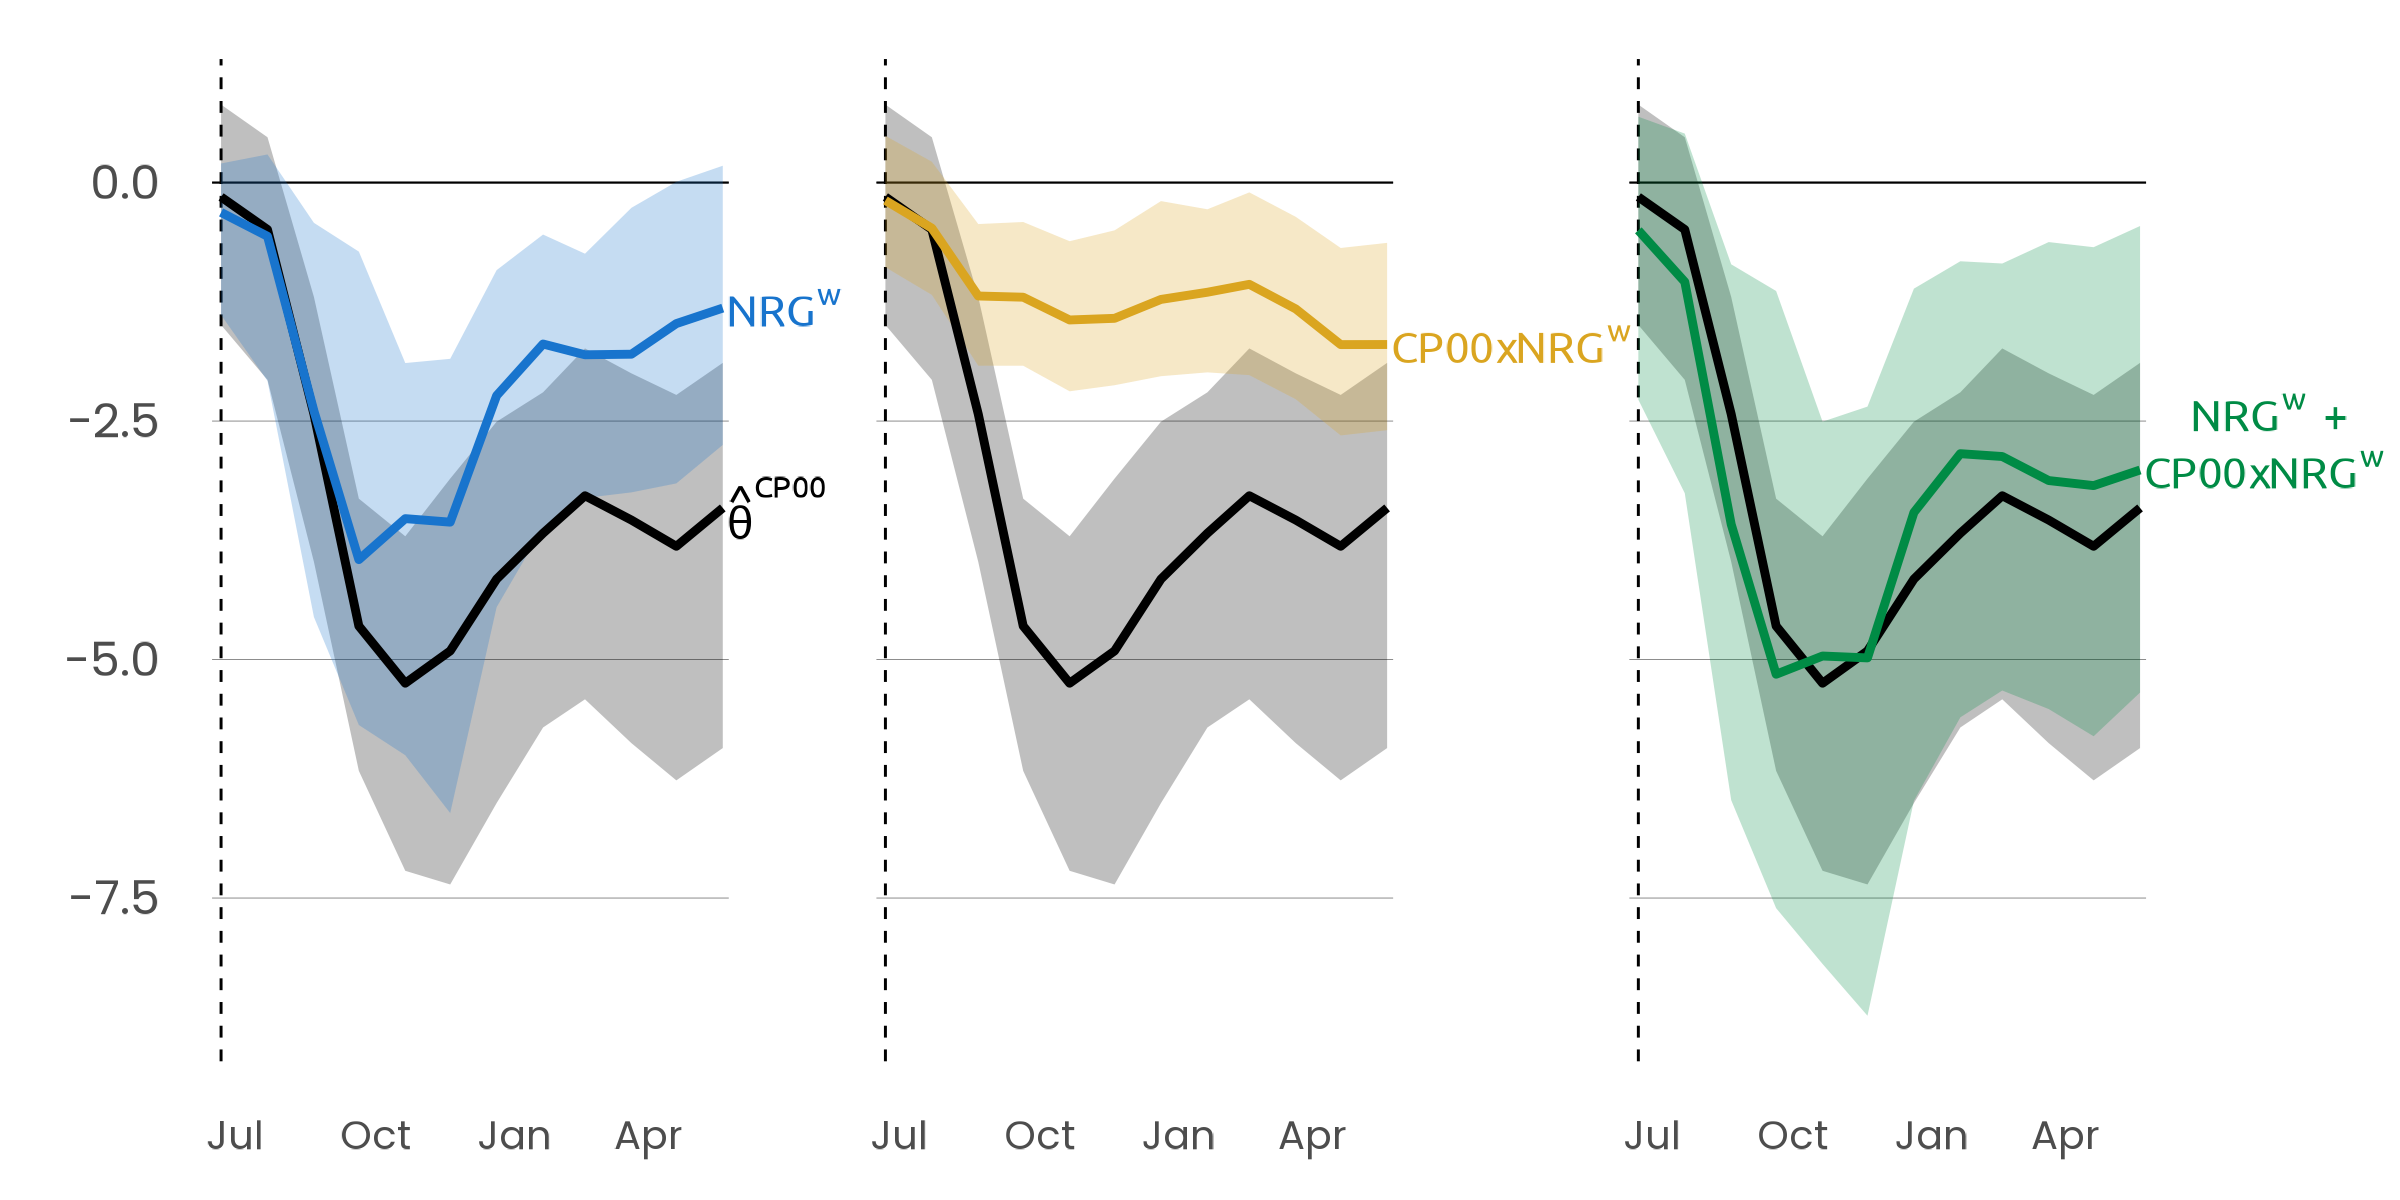
\includegraphics[width = .9\linewidth]{HICP_weights_12_ES.png}
    \caption{Decomposition of the effect on Spain’s overall CPI.}
    \label{fig:weighted_cp00_es}
\end{figure}
\section{Conclusion}
This paper has estimated the effect of the Iberian exception mechanism on consumer price inflation. In Spain, the intervention had an immediate and strong negative effect, as overall inflation was reduced by 3\% between July and December 2022. Throughout the first three months of the IbEx, the reduction in overall inflation is fully explained by the decline of the energy-only CPI. In the nine months that follow, as the effect of the IbEx spreads to non-energy goods and services, these are responsible for one-third of the effect on overall inflation. In Portugal, the effect of the policy kicked in with a six-month delay and achieved a 1\% reduction in overall CPI, mostly explained by a 14\% decline in energy inflation between January and June 2023. The explanation for the different results can be found in the retail electricity contract options available in each country. The regulated tariff in Spain creates a direct link between the wholesale price of electricity and the price paid by consumers, with immediate effects on inflation. By contrast, retail prices in Portugal reflect longer-term contracts.\par
The approach used in this study shows how Spanish consumer prices are highly exposed to fluctuations in the spot price of electricity in the short term. While the IbEx had a stronger effect on Spain's inflation, it must be noted that the energy crisis did not affect Portuguese consumer prices as much in the first place, as seen in figure \ref{fig:result_nrg}. Following this, it is advised that Spain revises the PVPC tariff to reflect electricity contracts with longer maturity as an effective way to shield consumers against future episodes of volatility in international gas markets. Furthermore, applications of similar price caps in other European countries are expected to have a delayed effect, as illustrated by Portugal. Another aspect to consider before implementing similar policies outside the Iberian peninsular is that any other European country has more cross-border interconnections than Spain or Portugal. As pointed out by \textcite{schlecht2022}, this can lead to larger outflows of electricity produced in the country implementing the price cap.\par
%\newpage
\printbibliography

\newpage
\appendix
\section*{Appendix}\label{appendix}
\setcounter{figure}{0}
\renewcommand{\thefigure}{A\arabic{figure}}
\setcounter{table}{0}
\renewcommand{\thetable}{A\arabic{table}}
\vspace{.25cm}
\begin{figure}[!h]
    \centering 
    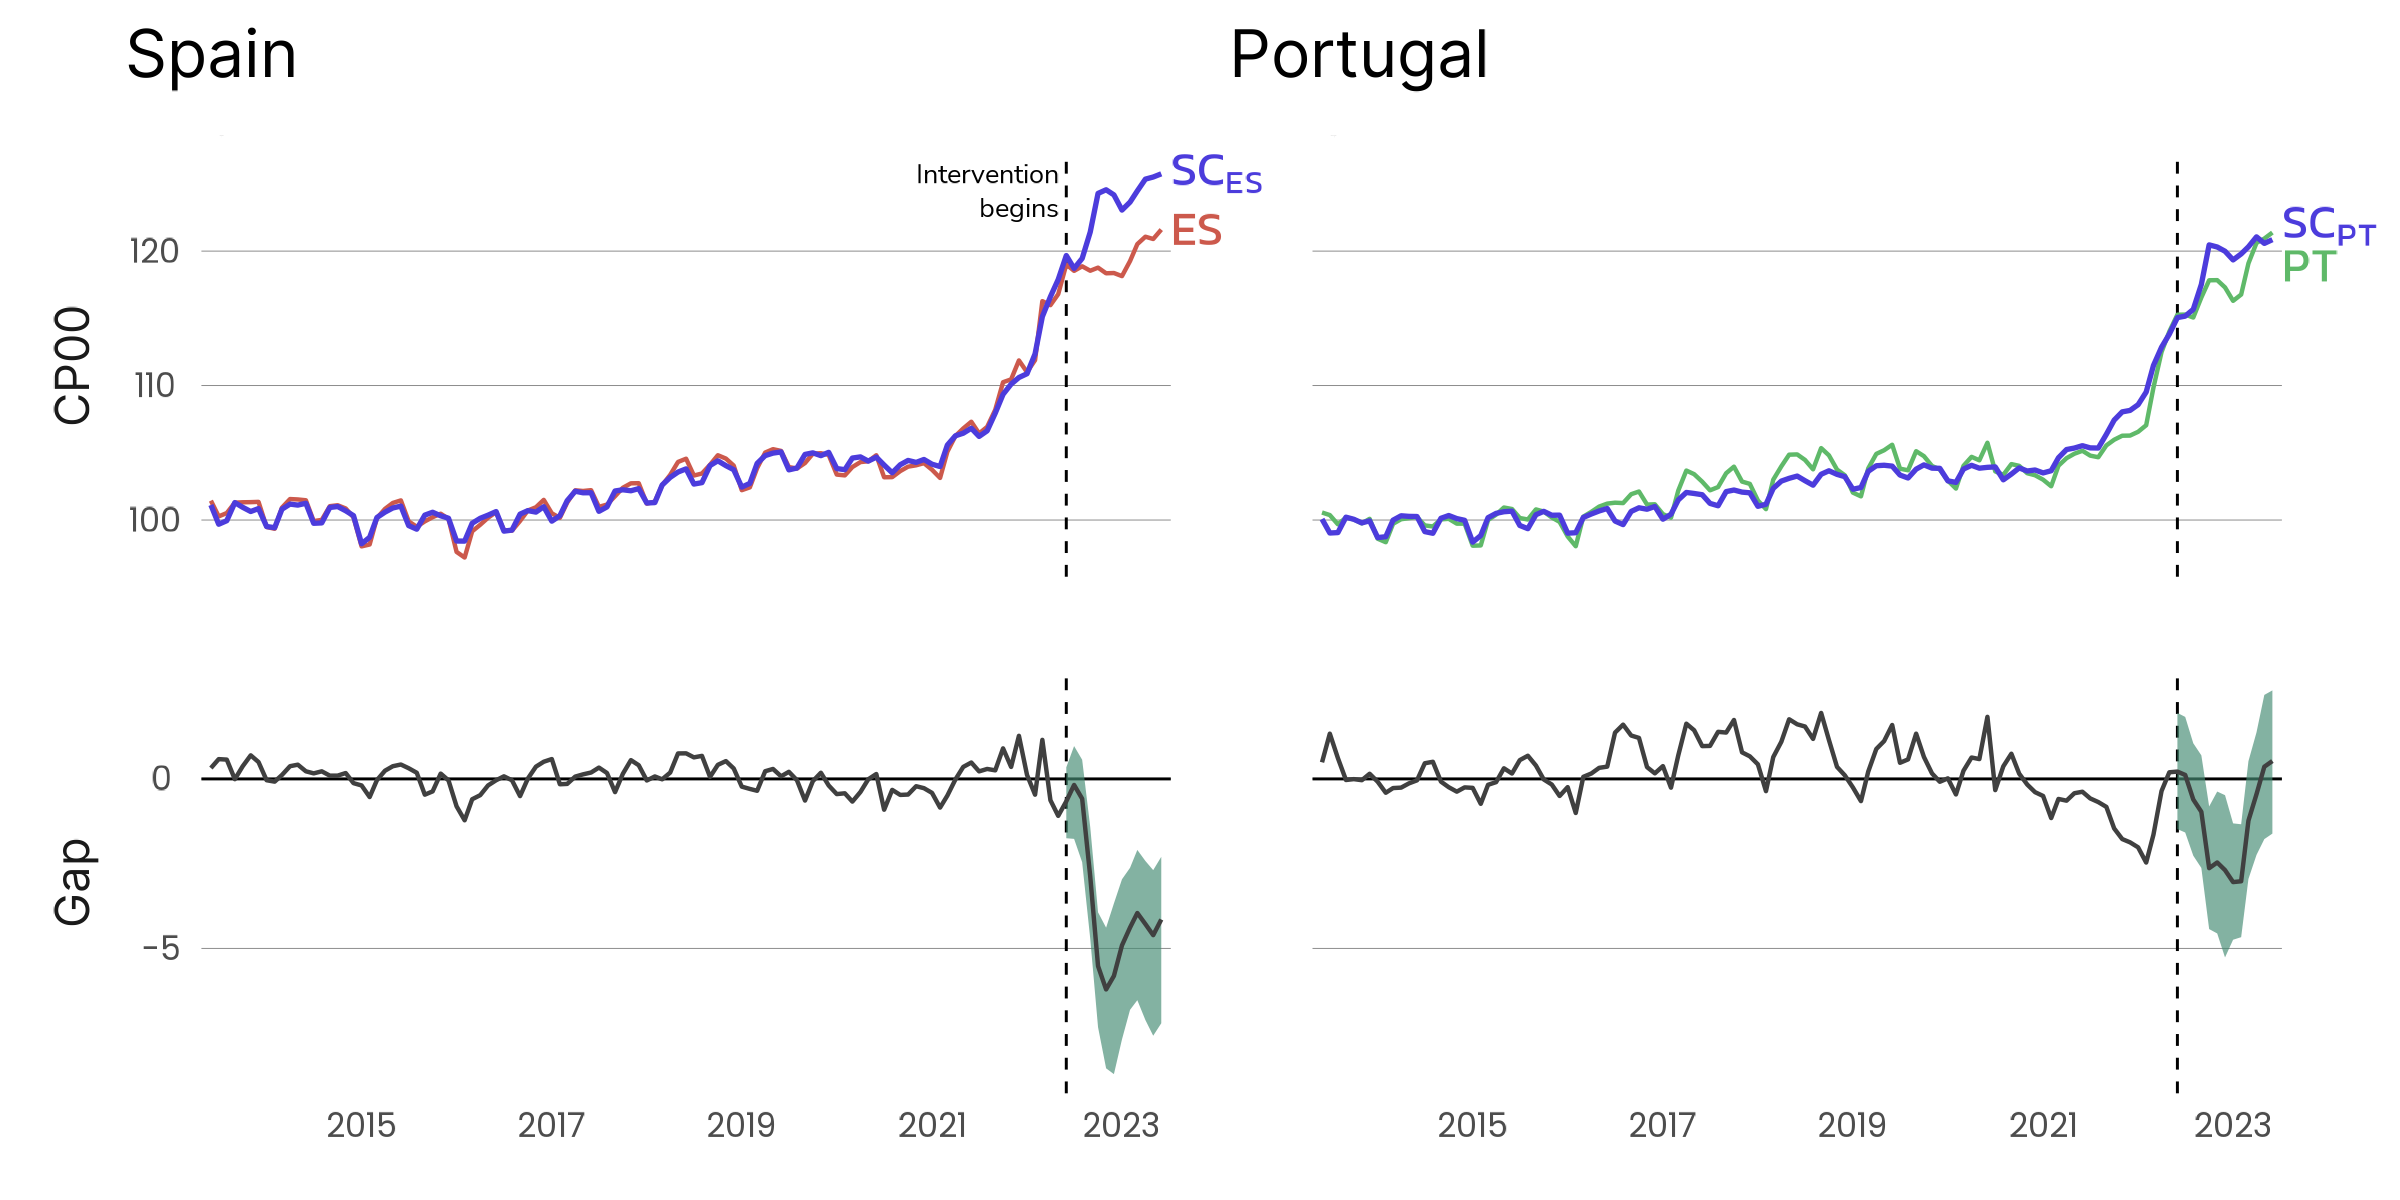
\includegraphics[width = .9\linewidth]{CP00_12_independent_y.png}
    \caption{Observed and synthetic overall inflation and difference between them with 90\% CI.}
    \label{fig:result_cp00}
\end{figure}
\vspace{2cm}
\begin{figure}[!h]
    \centering 
    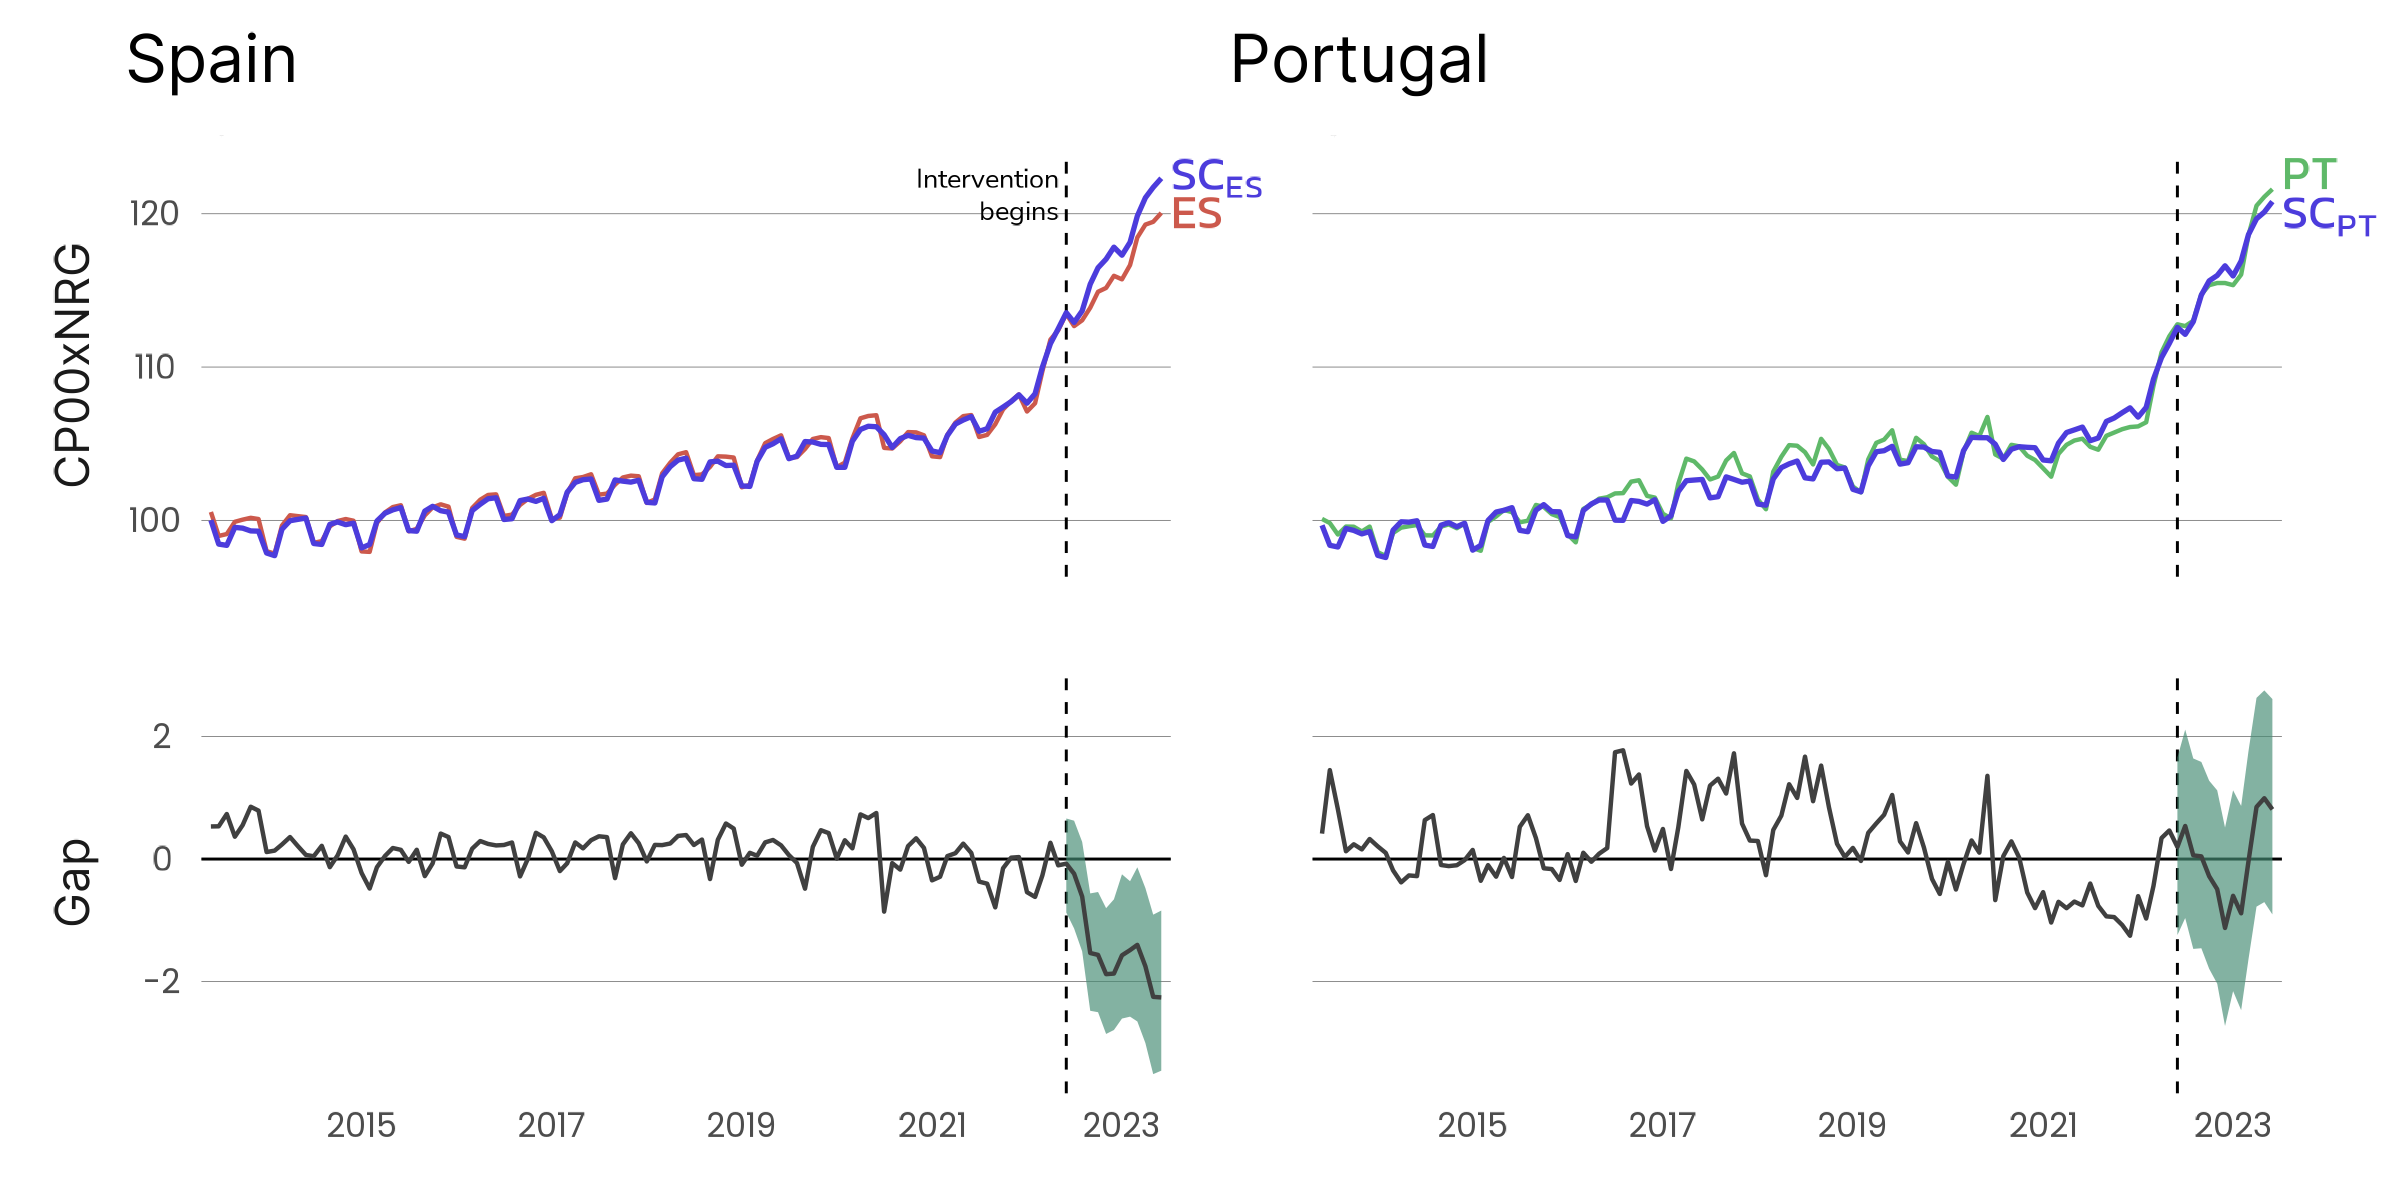
\includegraphics[width = .9\linewidth]{CP00xNRG_12_independent_y.png}
    \caption{Observed and synthetic overall inflation excluding energy and difference between them with 90\% CI.}
    \label{fig:result_cp00xnrg}
\end{figure}
\vspace{2cm}
\begin{figure}[!t]
    \centering 
    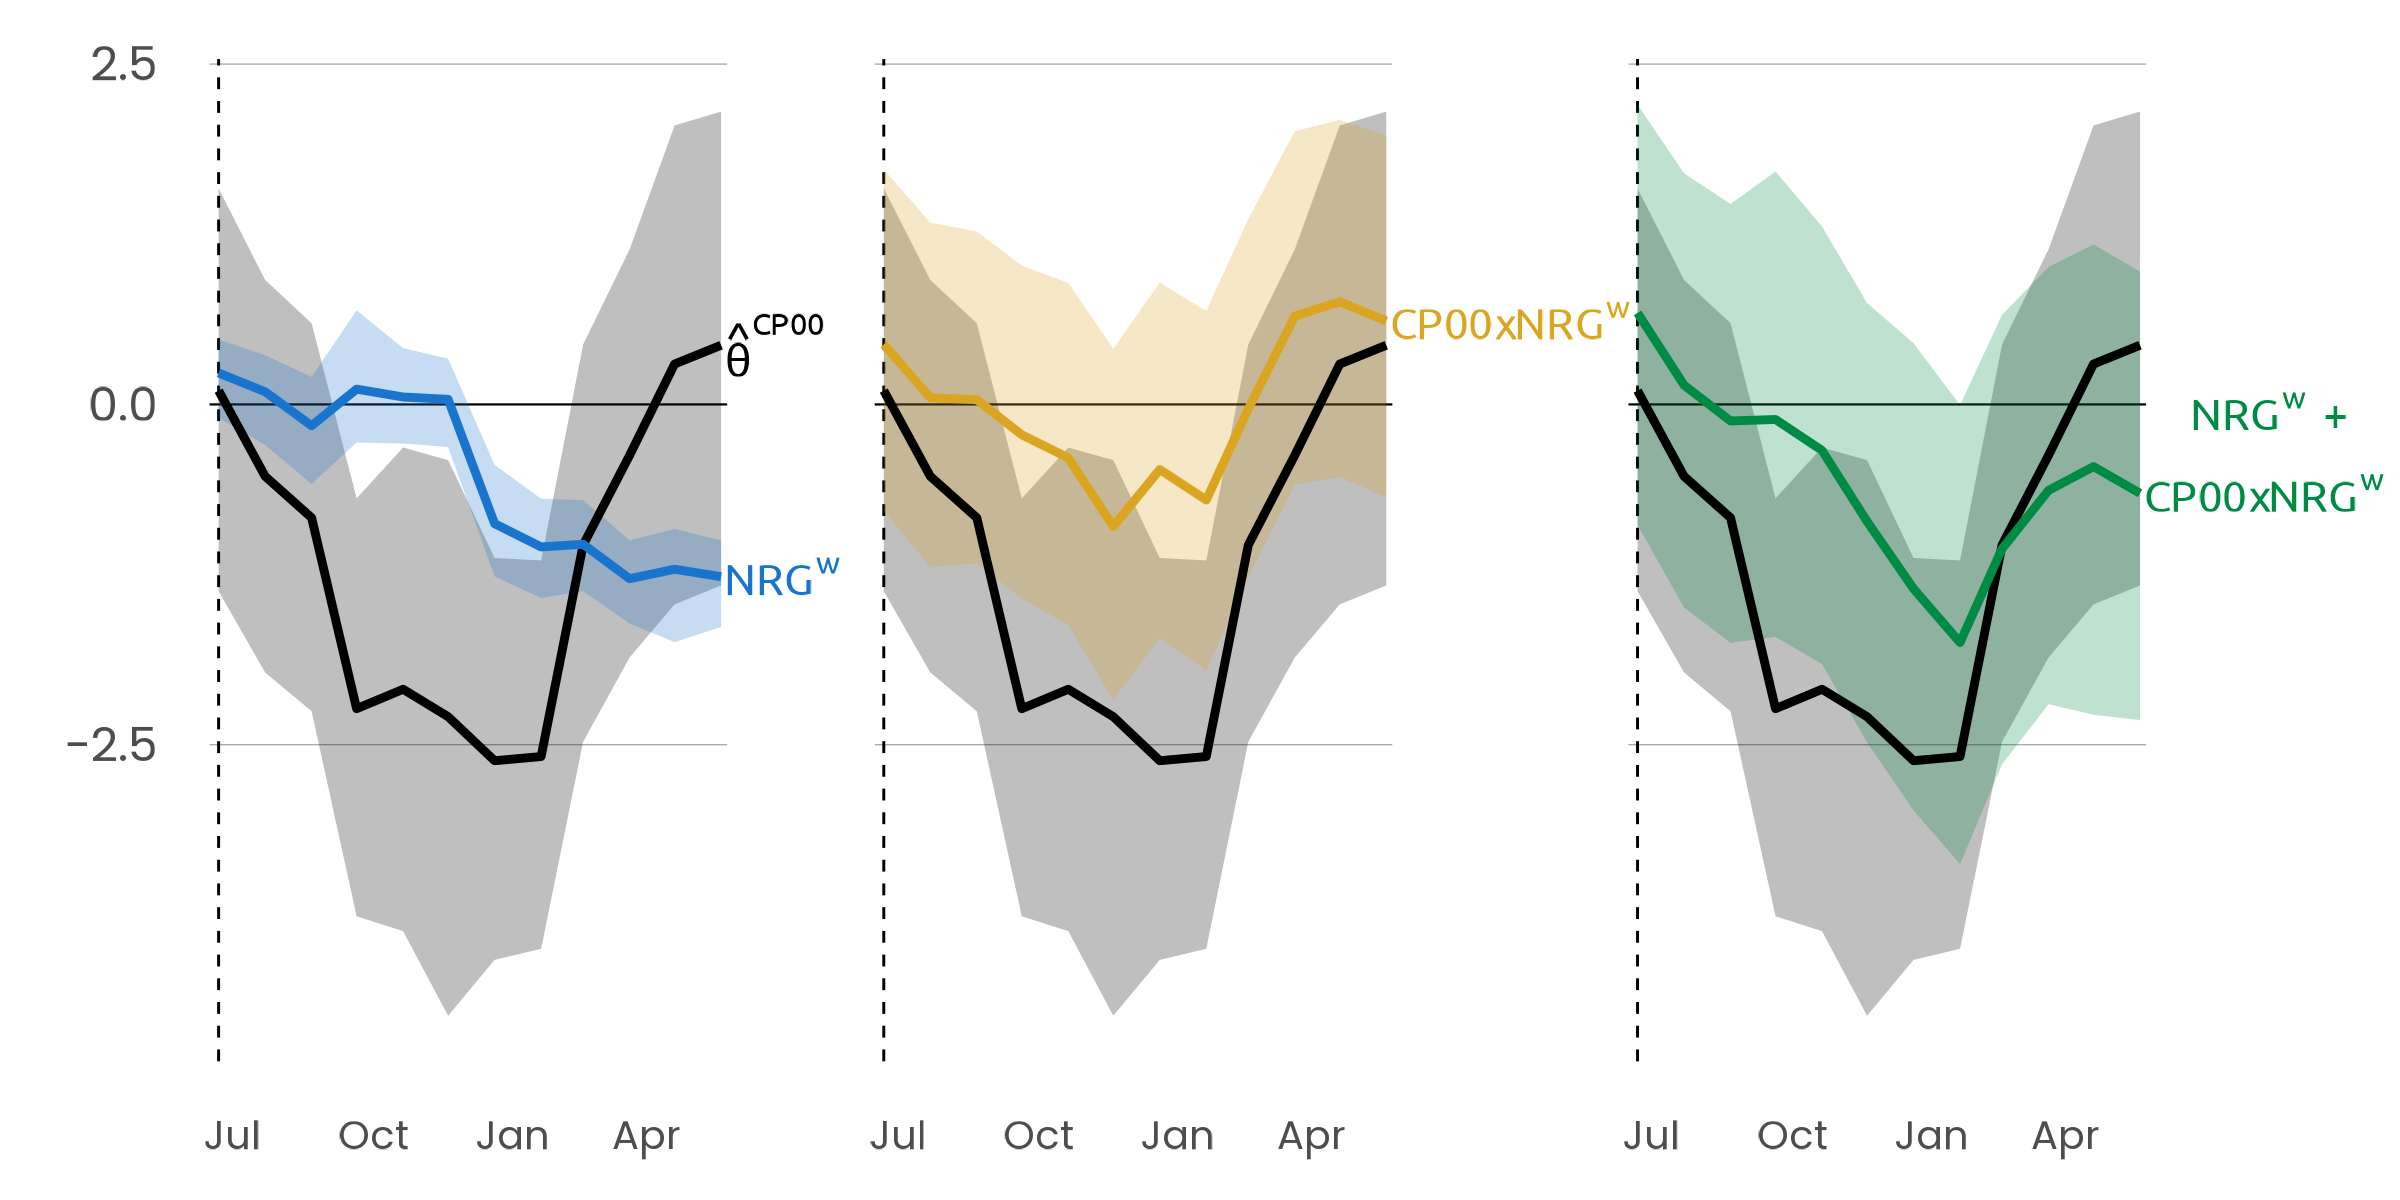
\includegraphics[width = .9\linewidth]{HICP_weights_12_PT.png}
    \caption{Decomposition of the effect on Portugal’s overall CPI. The weights for Portugal are .08023 (NRG) and .91977 (CP00xNRG) in 2022, and .08058 (NRG) and .91942 (CP00xNRG) in 2023}
    \label{fig:weighted_cp00_pt}
\end{figure}

\begin{table}[!t]
    \centering
    \setlength{\tabcolsep}{20pt}
    \renewcommand{\arraystretch}{1.35}
    \begin{tabular}{llccc}
        \toprule
        \toprule
        &  & Spain & Portugal \\
        \midrule
        DAA & Jul 22 - Dec 22  & -54.417 & -54.292 \\   
        &  & [-63.902, -46.286] & [-64.178, -45.931] \\
        & Jan 23 - Jun 23  & -33.64 & -31.883 \\       
        &  & [-46.669, -20.828] & [-46.101, -18.812] \\
        & Jul 22 - Jun 23  & -44.028 & -43.087 \\      
        &  & [-55.286, -33.557] & [-55.14, -32.372] \\
        \midrule
        NRG & Jul 22 - Dec 22  & -20.293 & 0.773 \\     
        &  & [-37.34, -6.227] & [-3.867, 5.154] \\     
        & Jan 23 - Jun 23  & -17.550 & -13.87 \\        
        &  & [-34.891, -3.89] & [-18.712, -9.828] \\   
        & Jul 22 - Jun 23  & -18.921 & -6.549 \\       
        &  & [-36.116, -5.059] & [-11.289, -2.337] \\ 
        \midrule
        CP00 & Jul 22 - Dec 22  & -2.979 & -1.313 \\    
        &  & [-4.713, -1.672] & [-2.952, 0.28] \\      
        & Jan 23 - Jun 23  & -3.646 & -0.98 \\         
        &  & [-5.951, -2.093] & [-2.536, 0.584] \\     
        & Jul 22 - Jun 23  & -3.313 & -1.147 \\        
        &  & [-5.332, -1.883] & [-2.744, 0.432] \\  
        \midrule
        CP00xNRG & Jul 22 - Dec 22  & -1.118 & -0.179 \\
        &  & [-1.929, -0.237] & [-1.516, 1.206] \\     
        & Jan 23 - Jun 23  & -1.508 & 0.145 \\         
        &  & [-2.505, -0.416] & [-1.224, 1.634] \\     
        & Jul 22 - Jun 23  & -1.313 & -0.017 \\        
        &  & [-2.217, -0.327] & [-1.37, 1.42] \\ 
        \bottomrule
        \bottomrule
    \end{tabular}
    \caption{Percentage treatment effect of the IbEx on day-ahead auction price, energy inflation, overall inflation and overall inflation excluding energy over different time periods.}
    \label{tab:ates}
\end{table}

\begin{table}[!t]
    \centering
    \setlength{\tabcolsep}{20pt}
    \renewcommand{\arraystretch}{1.5}
    \begin{tabular}{llccc}
        \toprule
        \toprule
        & & Spain & Portugal \\
        \midrule
        DAA & 7/2022 - 12/2022 & $<.001^{\ast\ast\ast}$ & $<.001^{\ast\ast\ast}$ \\
        & 1/2023 - 6/2023 & $<.001^{\ast\ast\ast}$ & $<.001^{\ast\ast\ast}$ \\     
        & 7/2022 - 6/2023 & $<.001^{\ast\ast\ast}$ & $<.001^{\ast\ast\ast}$ \\ 
        \midrule
        NRG & 7/2022 - 12/2022 & $<.001^{\ast\ast\ast}$ & .462 \\   
        & 1/2023 - 6/2023 & $.045^{\ast\ast}$ & $<.001^{\ast\ast\ast}$ \\         
        & 7/2022 - 6/2023 & $.014^{\ast\ast}$ & $<.001^{\ast\ast\ast}$ \\ 
        \midrule
        CP00 & 7/2022 - 12/2022 & $<.001^{\ast\ast\ast}$ & .239 \\
        & 1/2023 - 6/2023 & .376 & $.012^{\ast\ast}$ \\
        & 7/2022 - 6/2023 & $.057^{\ast}$ & $.067^{\ast}$ \\ 
        \midrule
        CP00xNRG & 7/2022 - 12/2022 & $.032^{\ast\ast}$ & .821 \\
        & 1/2023 - 6/2023 & .603 & .306 \\
        & 7/2022 - 6/2023 & .403 & .468 \\  
        \bottomrule
        \bottomrule
    \end{tabular}
    \caption{Resulting p-values from testing the null hypothesis of no effect of the IbEx on different outcomes.\\
    Note: * $p < .1$; ** $p < .05$; *** $p < .01$.p-values are computed via the iid method with 5,000 permutations \parencite{chernozhukov2021}}
    \label{tab:p_vals}
\end{table}


\end{document}
